\clearpage
\section*{三、数据处理与结果分析}

\subsection*{1. 内阻结果比较}

替代法测得内阻为 243 Ω，中值法测得内阻为 233.5 Ω，两者相差 9.5 Ω。两种方法的差异可能与总电流保持程度、读数及接触电阻有关，我主观认为的原因是：标准电流表精度有限，当电阻改变量较小的情况下，标准电流表示数均不变，导致电阻测量误差较大。

以替代法测得的 $R_g=243\,\Omega$ 设计电路，初始理论分流电阻为 $R_1=243/4=60.75\,\Omega$，理想等效内阻为 $R'_g=243/5=48.6\,\Omega$，对应理论分压电阻为 $R_3=1000-48.6=951.4\,\Omega$。这些是电路设计阶段的设计值。最终使用满偏校准后得到的 59 Ω、954 Ω，二者分别比初始设计值低 1.75 Ω、高 2.6 Ω，相对误差的绝对值分别为 $\approx2.88\%$ 和 $\approx0.27\%$，可以接受。


\subsection*{2. 校验曲线与仪表等级}

按课堂要求，示值误差取改装表读数减去标准表读数，即 $\Delta I=I_G-I_B$、$\Delta V=V_G-V_B$。以各校验点的最大绝对示值误差计算引用误差，再在课件列出的等级 0.1、0.2、0.5、1.0、1.5、2.5、5.0 中向上选取满足要求的等级。

电流表五点示值误差为 0.00、0.10、0.10、0.10、0.00 mA，最大绝对示值误差为 0.10 mA，故

\[
k_I=\frac{0.10}{5.00}\times100=2.0.
\]

最大引用误差为 2.0\%，介于 1.5 级与 2.5 级之间，向上取 2.5 级。

电压表在 2.00 V、3.00 V、4.00 V 三个校验点的示值误差均为 $0.10\,\mathrm V$，最大绝对示值误差为 $0.10\,\mathrm V$，故

\[
k_U=\frac{0.10}{5.00}\times100=2.0.
\]

按本次五个校验点，电压表最大引用误差为 2.0\%，评为 2.5 级。满偏点误差为零，只说明该点校准一致，不能据此认定整个量程无误差。

\begin{figure}[H]\centering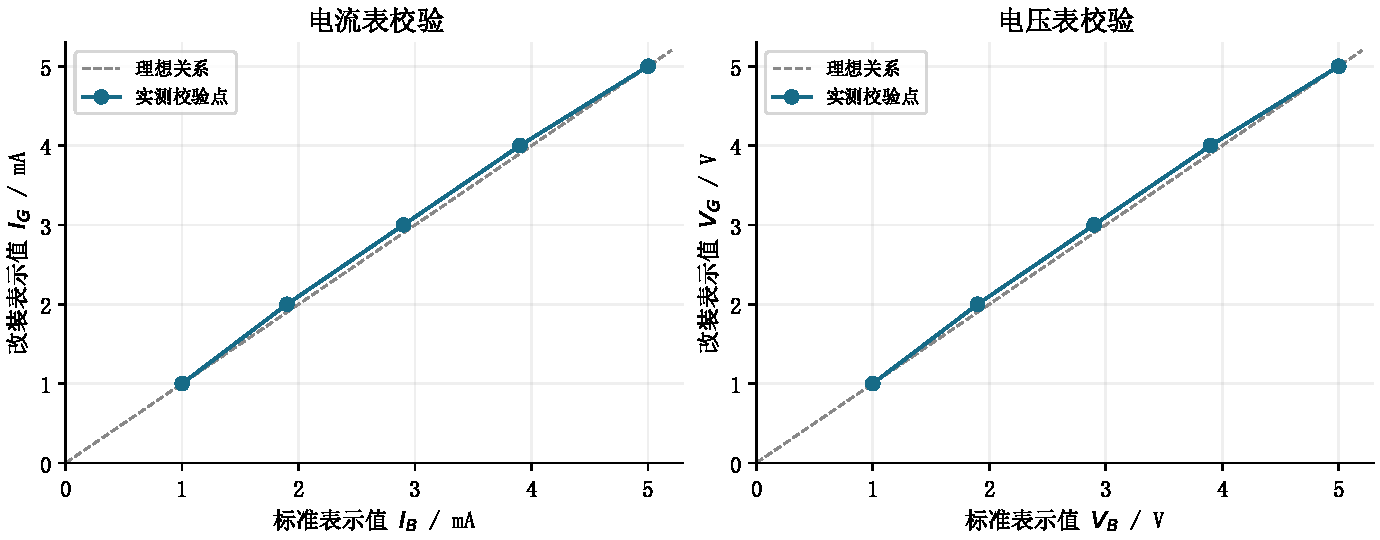
\includegraphics[width=.96\linewidth,height=5.1cm,keepaspectratio]{../assets/calibration.pdf}\caption{电流表与电压表校验曲线}\end{figure}

图中横轴为标准表示值，纵轴为改装表示值。连线仅用于显示相邻校验点的趋势，虚线为理想关系。中间校验点整体位于理想线上方，说明这些点的改装表示值偏大。

\subsection*{3. 欧姆刻度分布}

组装好欧姆表后，短接电路，调节调零电阻使得电流计满偏为 $I_0=1.00\,\mathrm{mA}$，实测 $R_x=300.0\,\Omega$ 时电流为 $0.50\,\mathrm{mA}$，故中值电阻为

\[
R_0=300.0\,\Omega.
\]

本实验记录的 $I_x$ 均为电流计支路的示值。保留分流支路时，电流计满偏示值为 1.00 mA，对应回路总电流为 5.00 mA。由标称电源电压估算，回路内阻为 $1.5\,\mathrm V/(5.00\,\mathrm{mA})=300\,\Omega$，与电流计半偏时测得的中值电阻一致。下式及图中的 $I_x$ 均表示电流计支路电流：

\[
I_x=\frac{300.0}{300.0+R_x}\times1.00\,\mathrm{mA}.
\]

\begin{figure}[H]\centering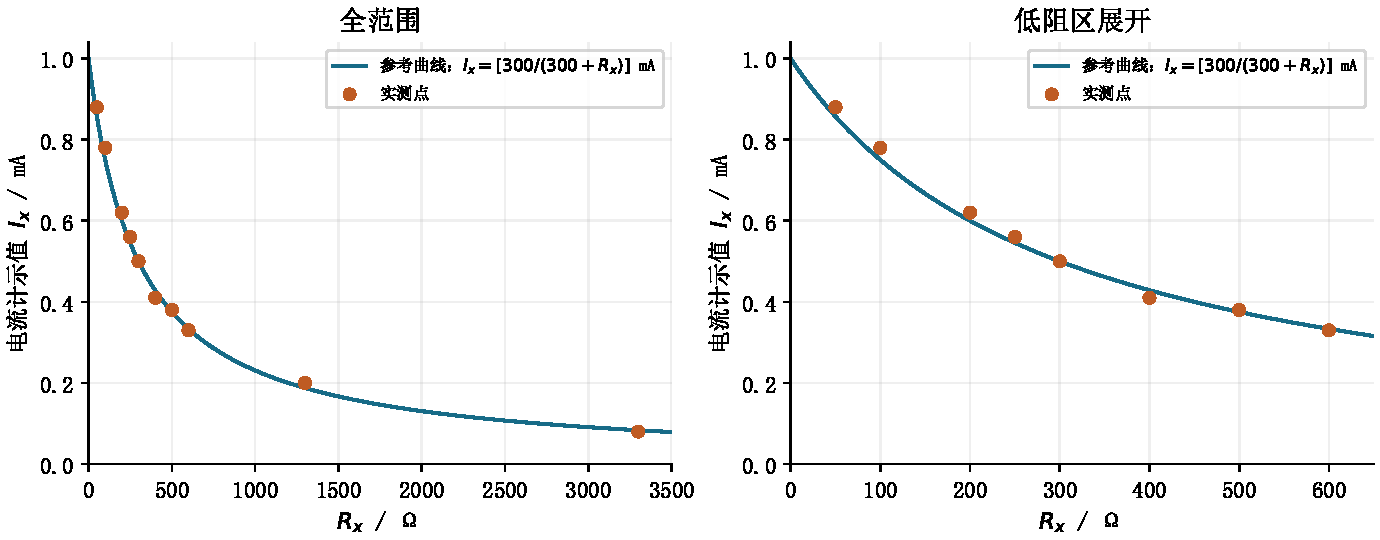
\includegraphics[width=.96\linewidth,height=5.6cm,keepaspectratio]{../assets/ohm-curve.pdf}\caption{欧姆表电流—电阻关系}\end{figure}

图中实测点随电阻增大而下降，整体接近参考曲线，实验测量结果较为满意。

\begin{figure}[H]\centering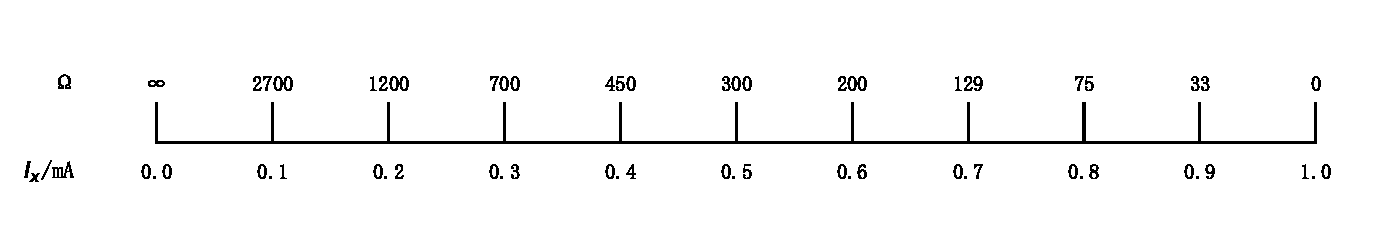
\includegraphics[width=.96\linewidth,height=2.2cm,keepaspectratio]{../assets/ohm-scale.pdf}\caption{按中值电阻 300 Ω 绘制的欧姆刻度示意}\end{figure}

图中按电流等间距标出对应的理论电阻。接近零电流时，微小的电流变化对应很大的电阻变化，因此高阻端密集；接近满偏时刻度较疏。

\clearpage
\subsection*{4. 误差分析}

\begin{enumerate}
\item \textbf{内阻测量：} 替代法和中值法的结果相差 9.5 Ω。替代法中，因为标准电流表的精度有限，电阻小幅变化时标准电流表示数可能仍不变，使“恢复原电流”的判断存在范围；中值法既要保持总电流不变，又要判断表头是否半偏，两次调节和读数都会引入偏差，所以也会存在一定误差。

\item \textbf{电流表与电压表校验：} 两表满偏点误差均为零，但中间三个校验点分别偏大 0.10 mA 和 0.10 V，说明仅调准满偏点不能消除全量程偏差。误差的其他原因还可能有：表头刻度非线性、读数视差，分流、分压电阻的实际阻值及接触电阻也会影响校准。

\item \textbf{欧姆表测量：} 高阻端的电流较小，如 3300.0 Ω 时表头仅为 0.08 mA，指针位置的微小判断差异就会导致电阻读数出现较大偏差。注意在测量之前，需要短接电路并调节调零电阻使得小表头满偏，否则会导致较大误差。总而言之，应在测量前短接调零，保证表笔接触可靠，并优先在中值电阻附近读数。

\end{enumerate}
